\documentclass[11pt,english]{article}
\usepackage[utf8]{inputenc}
\usepackage[T1]{fontenc}
\usepackage{babel}
\usepackage{biblatex}
\addbibresource{bibliography.bib}
\usepackage{graphicx}
\usepackage{float}
\graphicspath{ {./images/} }

% correct bad hyphenation here
\hyphenation{op-tical net-works semi-conduc-tor}
\begin{document}
\title{Use of Model-Driven Development to check for violations of the GDPR}
\author{
  Tijana Lalošević\\
  \texttt{tijana.lalosevic@uns.ac.rs}
  \and
  Gordana Milosavljević\\
  \texttt{grist@uns.ac.rs}
  \and
  Goran Sladić\\
  \texttt{sladicg@uns.ac.rs }
  \\Faculty of Technical Sciences,\\ University in Novi Sad, Serbia
}


\date{}
\maketitle


\begin{abstract}
The General Data Protection Regulation (GDPR) is a legal regulation on the use, protection and privacy of data issued by the European Union. Despite unification and centralization of law regulation, there is no universal software solution for automatization of checking GDPR compliance. Therefore, to overcome some security challenges, companies pay expensive manual checking executed by lawyers or create solutions that do not apply to other corporations and industries. In this paper, we discuss the data privacy challenges faced by companies in introducing the GDPR. To create a unified solution that would be applicable in all industries, we propose a solution in the form of a privacy meta-model, as also, OCL validations which provides automatic checking for violations of the arts of the GDPR. This meta-model represents the first step on the path of automatization of checking violations of the GDPR. Besides, we also present the results of our meta-model evaluation, alongside the case study of the bank which illustrates the usage of this meta-model.
\end{abstract}

\section{Introduction}

\quad The development of technology and the discovery of new technologies from the end of the 20th century and the beginning of the 21st century have brought extraordinary changes in many living fields. The introduction of techniques, computers and internet technology in everyday human life has helped to greatly simplify the business sphere, automating many business processes. It is automation that has contributed to saving the most important resource, time. It has led people to focus on their creative and work energy on more complex processes and learning and developing new skills instead of doing repetitive and often uninteresting jobs, which has implicitly led to a general increase in living standards. \newline As each age brings with it certain changes in the field of supply and demand, at the beginning of the 21st century, data imposed itself as the new 'gold'. As such, they have become interesting in the world of illegal activities. One of the main problems has become the leak of sensitive information and its sale on the black market. In addition, alterations and falsifications of data, theft of intellectual property and many other frauds became more frequent. Therefore, there is a need for the legal regulation of data use. Some of these regulations were: ISO 27001 \cite{iso}, ISACA's COBIT \cite{cobit}, Health Insurance Portability and Accountability Act (HIPAA) \cite{hipaa}, NIST "800 series" \cite{nist} and Payment Security Industry Data Security Standard (PCI) DSS) \cite{pci}.\newline Digitalization and social globalization have erased international borders and enabled the rapid growth and development of international business. Increased business movements have led to the problem of legislative inconsistencies between the countries in which it operates. This gap between regulations has made a place for many data thefts, resale and other abuses. To overcome this problem, the European Union adopted a legal framework, the GDPR \cite{gdprRegulation}. The GDPR was adopted on 14 April 2016 and became enforceable beginning 25 May 2018 \cite{gdpr}. This regulation aims to give individuals control over their data across the European Union and unify laws within the European Union to facilitate international business. It unified privacy management and data protection. It has brought many benefits to individuals, but also, it has provided many challenges and obstacles to companies and corporations that control or process personal data. On the business side, this regulation caused a great deal of difficulty. All companies had to adjust their business to the new rules in a brief period. \newline \quad Many surveys were conducted to determine how ready the market is for the new regulations. Based on Isaca survey \cite{isaca} the top five advantages related to GDPR compliance are:
\begin{itemize}
  \item Data discovery and mapping (59 per cent)
  \item Prioritizing GDPR compliance among other business priorities (47 per cent)
  \item Organizational education and change programs (45 per cent)
  \item Ensuring cross-departmental collaboration and buy-in (42 per cent)
  \item Preparation for data subject access or deletion requests (37 per cent).
\end{itemize}
\quad The Lipswitch survey \cite{lipswitch} has given the following results similar to the first survey. This survey reveals that 52 per cent of the examined companies admitted they were not ready to apply the GDPR, 35 per cent confessed to not knowing whether their IT policies and process were up to the job. Seo, Kim, Park and Lee \cite{8190804} have evaluated the economic impact on IoT under
GDPR. They examine which parts of Gordon and Loeb's defined costs \cite{gordon2002economics} are expected to change due to GDPR, as is shown in Figure 1. They estimated the company’s costs for each of these four types, as is shown in Figure 2.
\begin{figure}[htp]
    \centering
    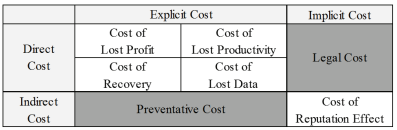
\includegraphics[width=6cm]{costs}
    \caption{Gordon and Loeb Model’s Cost that GDPR affects}
    \label{fig:costs}
\end{figure}
\begin{figure}[htp]
    \centering
    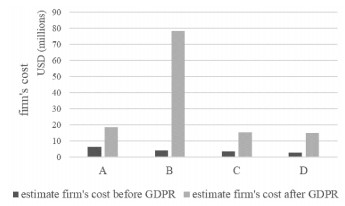
\includegraphics[width=6cm]{comparation}
    \caption{Comparison of company’s costs before and after GDPR}
    \label{fig:comparation}
\end{figure}
\newline These results are not unexpected, as it is the main cause for that is a lack of a single comprehensive solution that would be applicable and easy to integrate into all technologies. The secondary cause was a misunderstanding of terms and expressions which have come with the GDPR. Therefore companies are most often forced to pay legal experts to study their business ecosystem. After this step, companies pay the IT team to design a unique solution for their information system based on those studies. As we notice, the whole process is slow, expensive, and errors prone. \newline This paper aims, above all, to reduce costs by implementing a unified solution that is usable in any industry. We exclude the need for additional legal interpretations and the implementation of a customized solution for an individual client. Our first goal is to create a universal meta-model that is close to natural language, which excludes the need for further interpretation of terminology. This meta-model can describe the real scenarios of using personal data in the information system and check whether their usage follows the GDPR. The idea is for this solution to be usable in any industry. Whether we are talking about the banking, medical or transportation sector, it is possible to map the entities listed in the meta-model to the desired business domain. It avoids the need to adopt the solution to a particular business domain. To achieve this goal, we used Model-Driven Engineering (MDE) technologies \cite{mde}, such as UML \cite{uml} and Object Constraint Language (OCL) \cite{ocl}. After that, we will examine the expressiveness of the meta-model and the usability of OCL validations on the example of the bank case study. Finally, as it is the first step towards easy integration with software solutions and automatical verifying compliance of business processes to the GDPR, we will introduce our strategy for future development. \newline The structure of the paper is as follows. In the second section, we provide the related work. In the third section, we present our meta-model with accompanying OCL validations. After that, in the third section, we demonstrate the usage of the meta-model on the example of a bank case study. In the fourth section, we discuss the results and limitations of the study. Finally, in the last section, the paper has been concluded, and some future development has been proposed.
\section{Related work and Discussion}
The GDPR is considered the toughest and rigorous privacy and security law in the world. The fact that it includes all manipulations over the data manifests its complexity. Starting with data collection, storage and transformation, transport, processing and ending with stop processing. It places special emphasis on the data owner and the role he assumes in data processing. The data owner is the only one who can manage the data, introducing terms such as complaint, withdrawal of consent and request for the erasure. We can see how comprehensive the GDPR is in that it covers all previously adopted regulations and safety standards. During their validity, numerous software solutions were designed. Although no specific standard or universal solution was established even then, because even then the companies had an almost identical approach to solving the problem, it is important to analyze these solutions as well. As old solutions have proven to be beneficial and have been used in use for many years. So, they can therefore serve as a starting point for research.  They can also serve as a good reference point for analyzing the limitations of existing solutions.
\subsection{Earlier regulations}
Since digitalization prevailed, the data became more accessible, so the software became more susceptible to software attacks. To define a certain standard for data protection, states regulated them by law. Due to the large amount of personal data they handle, the IoT \cite{iot} and health systems have stood out as the most attractive targets for hacker attacks. Considering the nature of these systems, they required automation of processing and collection of data. According to this, most of the previous research has been concerned with finding solutions for them.\newline The first hurdle the industry faced was data encryption. Hence, Ding and Klein \cite{encryptionLevel} propose a novel model-driven application-level encryption solution to protect the privacy and confidentiality of health data. They suggest the cooperation of domain experts, who specify sensitive data, and security experts, who determine cryptographic parameters, thus creating the security configuration. After that, the code generator generates code and configuration artefacts to control the encryption and decryption logic. The disadvantage of this paper is that it is closely related to data encryption, but its contribution is in the very cooperation of different experts to define a domain-specific language and limitations that will be clear to both parties. This is exactly what I wanted to achieve during the modeling of the solution so that all concepts and their interrelationships would be clear to both legal entities and software engineers. On the other side, Amato, Flora, and Moscato suggest a different approach. In their first paper \cite{6245777}, they introduced MetaMORP(h)OSY methodology and framework. Then, they present the solution \cite{amato2015model} based on lifecycle validation. They extend the MetaMORP(h)OSY modelling profile to explicitly consider privacy requirements for data. Authors specialize the stereotype for every role in the health system. After that, they create a data lifecycle with predefined states containing semantics. Then, they implement a translation algorithm to perform verification at every lifecycle step. This solution is flexible on the part of the end-user who can independently define the validation behavior in each state, however, this is exactly his flaw since he can easily make a mistake when manually filling in the state. Unlike the aforementioned paper, this paper deals with data access rights in addition to data encryption but does not support the handling of juvenile data, as well as the possibility of complaints from data owners. \newline Rahmouni, Solomonides, Mont and Shiu \cite{rahmouni2011model} were the first to acknowledge the problem with the different rules governing privacy protection. Their proposed solution is an ontology-plus-rules based approach to privacy decision support. Their target group was health systems across Europe. Their solution uses the Web Ontology Language (OWL) \cite{owl} to represent privacy rules in the context of medical data. Choosing the OWL has several advantages. It enables overlapping model concepts, even when legal objects use a different naming convention for the same resource. However, the OWL cannot solve complex legal rules based on if-else logic. In this case, they used the Semantic Web Rule Language (SWRL) \cite{swrl} for them. This solution has been contemporary and comprehensive, as it allows easy expansion and support for new regulations. They were among the first to acknowledge the concept of consent and the purposes of data processing. Through evaluating phase, they focus on the health system from states which are part of the EU, like the UK, Italy and France. The most relevant requirement was patient consent for two critical phases of the data lifecycle, as uploading the data and sharing the data. However, the disadvantage of this solution is primarily that it is closely related to the use of medical software. It also does not include the concepts of complaints, changes and withdrawals of consent, as well as the mechanism of informing users, which are one of the basic requirements of the GDPR. \newline  Anacleto, Antonio and Filomena \cite{correia2017model} proposed one of the first generic solutions, which can be applied to any information system. Namely, their solution is based on the use of a model-driven approach. The process itself begins with a domain-specific language, which is based on the vocabulary present in the standard itself. OCL validations are then performed on this model to verify compliance with the standard. After which the transformation into a platform-specific model is performed. Unfortunately, this paper does not provide a meta-model of a domain-specific language, which would really have value for further analysis. What gives value to this solution is that it is platform-independent and therefore generic. However, the disadvantage is that you still have to use a domain-specific language and use a specific model that will be validated, which is almost impossible in practice. Unlike the proposed solution, which aims to automatically create models. In addition, Ivan, Zlatogor and Rumen presented MDA information systems design \cite{gaidarskimodel}. Their solution focuses on data processing. Based on the domain-specific language, they transform a specific model into a UML model, then allow the user to define the validation itself using activity diagrams, after which they generate solutions on a specific platform. This solution is completely flexible, except that the validation is not defined on the meta-model itself, but is left to the DSL users themselves, which does not solve the problem of misinterpretation of regulations. Also, this solution is closely related to the use of data, not to their transfer or possible complaints by data owners.
\subsection{GDPR}
One of the significant technic breakthroughs after the discovery of the Internet was cloud computing. Cloud computing presents the delivery of different resources as applications, data storage and databases through the Internet. On the one hand, it proves a new level of flexibility and scalability. On the other hand, it brings new security and privacy challenges. \newline Opara, Song, Cho and Chung addressed these challenges in an extraordinary way. They introduce CERBERUS \cite{opara2019representing}, a framework for representing multi-cloud security and privacy policies and detecting potential problems in the security policies. CERBERUS consists of DSL, which is extremely easy to use and close to natural language. What makes this DSL simple is the use of pronouns and adjectives, such as who, why and when. Precisely because of this, it is easy to understand even for people who know nothing about the legislation or privacy models. It uses two categories of security policies, authorization (A) and obligation (O). After creating a specific instance, it looks for inconsistencies in access rights and thus validates the model. Barati and Rana \cite{barati2020tracking} represent a solution for cloud privacy that uses blockchain technology for auditing purposes. They created the GDPR Contract Factory. This factory generates four smart contracts (compliance, user consent, container and verification contract) that provide the basis for the verification of actor operations and privileges. Each of these four contracts answers one of four legal questions, which are defined earlier in the paper \cite{corrales2018smart}. 
\begin{itemize}
    \item Legal question L1: relates to the sensitivity of user data. In the GDPR standard, sensitive data consists of information, such as religious or political beliefs, genetic data, biometric data and health-related data.
    \item Legal question L2: checks if cloud services have a user
authentication mechanism.
    \item Legal question L3: verifies the geographical location of a
provider receiving user data.
    \item Legal question L4: checks for Binding Corporate Rules
(BCR) certification of non-European data receivers. The BCR is a code of conduct adopted by a community of multinational companies that want to move user data internationally across various jurisdictions.
\end{itemize}
They evaluate the presented solution on the example of the pharmacy service hosted at a cloud data centre. The disadvantage of this solution is that it is closely related to cloud computing and has a small set of user actions, as read, write, transfer and profiling user actions. On the other side, Michael, Netz, Rumpe and Varga \cite{michael2019towards} presented an interesting solution that is not strongly related to the IoT. They implemented a privacy meta-model with graphical language and a code generator. Code generator uses a specific model for input and generates the system code. The crucial concept in this meta-model is PrivacyPolicyRule. Through this concept, the user can define his own rule for the usage of his privacy data. This concept includes information as to which data are used, who is collecting them, where are they will be stored and in which period. \newline Feltus, Grandry, Kupper and Colin \cite{feltus2017model} express a new perspective on privacy management and its adjustment to GDPR. They propose a privacy meta-model and discuss how it can help understand privacy management in affiliated companies. This meta-model relies on RBAC and defining access rights within the organization. As is expected, the core concepts are Role and Resource. They define the RBAC model with extension, so the owner of data has the privilege to remove action, which other users perform on their data, at any time. With this extension, they introduced the concept of withdrawal consent. The concept resource has important information, for example, that it needs additional security protection or who collects this resource. \newline There are several different representations of DSL in the literature we most often encounter graphic and textual representation. Vanezi, Kapitsaki, Kouzapas, Philippou and Papadopoulos \cite{vanezi2020dialogop} give a terrific example of a graphical tool for formally defining GDPR purposes. This graphical tool is intuitive. Its syntax is similar to the syntax of the BPMN diagram. The disadvantage of this paper is that it deals only with the concept of purpose, so nowhere does it deal with the rights of data owners, such as consents, appeals, withdrawals of consent and other crucial terms provided by the GDPR. Caramujo, da Silva, Monfared, Ribeiro and Calado \cite{caramujo2019rsl} created DSL for the rigorous specification of privacy policies and implemented textual representation based on the Xtext framework \cite{bettini2016implementing}. This DSL is flexible and straightforward. The advantage of this work is that it is intended for cloud use because it anticipates the concept of the service and sub-service. The most specific concept in this DSL is Enforcement. This concept supports additional rules for data usage (e.g., check whether people under 13 years old should not use the service). They confirm the solution by comparing the policies guidelines from Facebook, LinkedIn, Twitter, Dropbox and IMDb. \newline It is interesting to see the analogy between the \cite{torre2019using} and our approach. This solution was only an introduction to the next research  \cite{modeldrivengdpr} which is not published yet. This solution provides a complex and comprehensive meta-model of GDPR. During development, the authors collaborated with legal experts to address as wide a range of GDPR acts as possible and translate every legal term into the model entity. After the design phase, they translate acts into the OCL rules. This DSL is very detailed and introduces many mechanisms for property rights support. Also, this research deals with supervisory authorities, legal liability and penalties. This solution provides OCL validation for almost all GDPR acts. The disadvantage of this paper is that it requires great expert knowledge in the area of legislation, and it does not provide for use in cloud systems.
\section{Privacy meta-model}
Complexity, dynamism and interdependence rules defined by the GDPR emphasises the need for a comprehensive modelling approach that abstracts this complexity and allows unambiguous validation of the business process. To adequately describe user behaviours within business systems, it is necessary to model actual systems. During modelling, in addition to the context and purpose, it is important who is the targeted audience. Hence, the biggest motivation for this research was to make a comprehensible DSL that will be easy to use for people who are not lawyers or legal experts. In the first step towards automatic validation of GDPR, we build a generic model representing the GDPR. This modelling activity involves defining a UML class model that encompasses key GDPR concepts and coding a set of OCL constraints.
\subsection{Main concepts}
We overview this meta-model by summarizing its main concepts: NamedElement, PrivacyPolicy, PolicyStatement, PrivacyData, SharedPrivacyData, Principal and Purpose. These elements represent the foundation for further development and validation. Figure \ref{fig:mainconcepts} depicts these concepts. Throughout the following sections, we will present each of these elements. After that, we will give an insight into the complete model and all other elements and their mutual relationships.
\subsubsection{NamedElement}
A NamedElement is one of the typical elements of every domain-specific language. It is an abstract class that provides a name for every element which inherits it. In modelling a domain-specific language, the concept of a name uniquely identifies specific instances.
\subsubsection{PrivacyPolicy}
A PrivacyPolicy element describes a central concept of this meta-model. It contains information about the specific company whose business system we want to validate. Reference on the owner represents this information. Also, it is a container of all the elements of the meta-model. Besides this, it includes additional information on the security controls used in this system. It will be explained below when we introduce other concepts.
\begin{figure}[H]
    \centering
    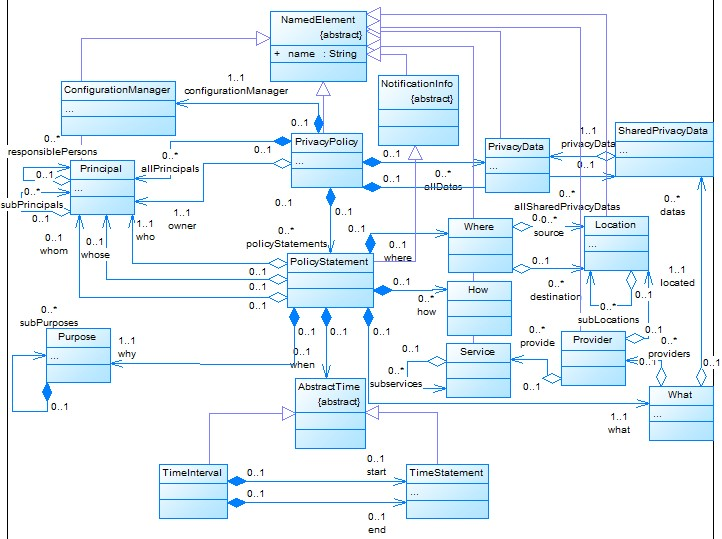
\includegraphics[width=12.5cm]{images/mainconcepts.jpg}
    \caption{Main concepts}
    \label{fig:mainconcepts}
\end{figure}
\subsubsection{PolicyStatement}
A PolicyStatement describes the actions of users in a certain period. Basically, it represents the unit whose validation we want to perform. It inherits class NotificationInfo, but more on this later when we talk about notifications. To make DSL as understandable as possible, it should use prepositions and adverbs from natural language to describe the details. A What element provides the information about what actions are performing. A PolicyStatement has information about when the action occurs. For this purpose, the abstract class AbstractTime represents time through a specific moment or a time interval. A How element describes which documents were provided to perform the specified action in the system. This will be described in more detail in the Documents section. A Where element provides information about the source and destination of the user's action location. A Purpose has information on why users use a PrivacyData. Also, PolicyStatement contains information on who perform actions, whose PrivacyData are over which actions are performed, and if PrivacyData transfer is performed, to whom the specified data is sent.
\subsubsection{PrivacyData}
The PrivacyData element describes a type of processed data in the business system. For example name, surname, email address and bank account. It inherits the NamedElement, as is presented in Figure \ref{fig:mainconcepts}. The SharedPrivacyData element represents the concrete user's data. It provides information about used additional security mechanisms on the specific data. Besides, the SharedPrivacyData contains information about the source and if this data is collected from the owner. The GDPR requires these two pieces of information about the data source through Article 14.
\subsubsection{Principal}
The Principal element defines the user in the business system. Like PrivacyData, it also inherits NamedElement. It supports grouping other principals in the group and defines rules for them, for the same reason it owns a collection of the subPrincipals. Also, it provides additional information such as PrincipalType, which describes the Principal as a legal entity or natural person. The PrincipalScope defines the Principal as a company's member if it belongs to the in-scope, to an external person if it belongs to the out-scope or an undefined group. Depending on which group it belongs to, the user has different access rights. In addition, the Principal has information on the age of the user. 
Reasons for that are Articles 3 and 8. These articles require that minors should be treated specially. Based on Article 8, each state has the right to define its age limit. If the state has not defined an age limit, the EU considers the child is below the age of 16 years. It is for this reason that Location contains information about this limit, as is presented in the Figure \ref{fig:purpose}.
\subsubsection{Purpose}
A Purpose is a primary element required by the GDPR. Provides information about why a particular user is using a PrivacyData. It has defined a reason and subreason as mandatory fields and optional free text field details so users can describe the purpose. ProcessingReason is a predefined list of values. Based on the selection, the user gets a ReasonSubtype list with predefined values. During data collection, the user defines the purpose for data collection. Also, the user specifies the allowed purposes for data processing. To model this and be able to perform validation, the purpose contains a collection of subpurposes. 
\begin{figure}
    \centering
    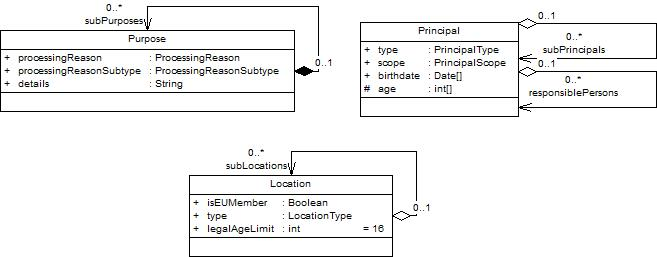
\includegraphics[width=12.5cm]{images/purposeAndPrincipal.jpg}
    \caption{Purpose, Location and Principal details}
    \label{fig:purpose}
\end{figure}
\subsubsection{Location}
A Location defines a specific geographical location. As is prescribed in Article 1, the GDPR applies exclusively to the member states of the European Union. Also, the European Union treats transfers to countries outside separately. Precisely because of this, the Location entity contains information on whether it is part of the EU. As the Principal, it inherits NamedElement and supports grouping other locations in the group. Through grouping entities, users can define general rules. A LocationType determines the type of the Location as union, country or region. It adds flexibility to the model and allows the user to specify rules based on the  Region itself.
\subsection{Details concepts}
After a detailed presentation of the main concepts, we will give a detailed overview of other entities of this meta-model. To make the purpose of each entity clearer, we also list the articles of the GDPR based on which we performed modelling.
\subsubsection{Configuration}
A ConfigurationManager provides the possibility to the user of the specific informational system to configure peculiar protection controls and data sources, 
which depend on the context and technology used. It makes the domain-specific language more adaptive and flexible. Some of the examples for the ProtectionControls are OriginalData, Encryption and Pseudonymisation, and for the DataSources are PubliclyAccessibleSources, Internet and SocialNetwork. As general protection control rules, PrivacyPolicy defines a sub-set of already specified protection controls from the ConfigurationManager. So, every SharedPrivacyData supports the definition of specific rules for specific data. It prop-ups the possibility that each exact data may have additional protection if the data owner explicitly demands it. Besides this, Article 14 prescribes that every data in the system should have defined the origin. For this reason, we modelled a SharedPrivacyData as a separate entity. It contains information about data sources if the data is not collected directly from the owner.
\begin{figure}[H]
    \centering
    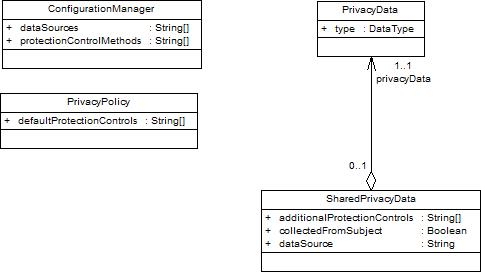
\includegraphics[width=10cm,scale=0.5]{images/configuration.jpg}
    \caption{Configuration details}
    \label{fig:configuration}
\end{figure}
\subsubsection{What and Time}
The What is one of the prime entities in the meta-model, so it is a mandatory element. At first, it defines performed actions in the system. Then, it provides support in case the information system's infrastructure is based on the cloud. In this case, it is possible to define which providers provide which service. Also, if the cloud infrastructure groups the services into specific subgroups, this can be described using subservices. As the GDPR specifically treats data transfers outside the EU, the provider also has a defined location. \newline The Time entity gives a temporal dimension to the meta-model, allowing it to perform validation depending on the chronological occurrence of privacyStatements. As the user defines time as a moment or time interval, we modelled the time as follows. TimeStatement and TimeInterval inherit class AbstractTime. TimeStatement defines a specific moment at the time. TimePreposition places the TimeStatement in a specific moment of the time. TimeInterval defines interval using start and end TimeStatement. We defined OCL validation to ensure that the user used prepositions in a correct and meaningful way. Later meta-model checks where we check if privacyStatement executed before or after the other privacyStatement, also rely on time prepositions.
\begin{figure}[H]
    \centering
    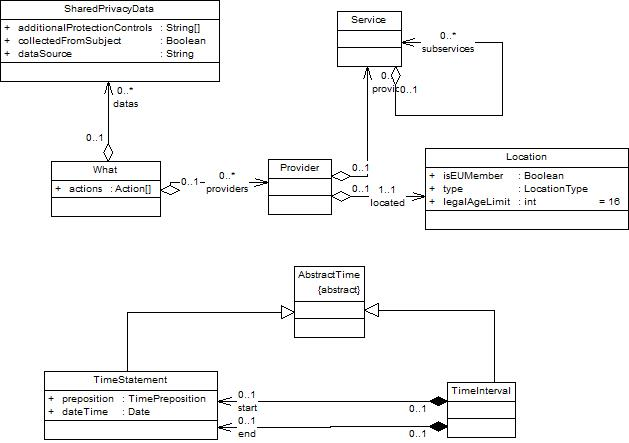
\includegraphics[width=10cm,scale=0.5]{images/whatAndTime.jpg}
    \caption{Detailed view of the What and Time entities}
    \label{fig:WhatAndTime}
\end{figure}
\subsubsection{Documents}
The GDPR focuses on data owners. With this in mind, we introduce the concept of consent. Articles 6 and 7 clarify the consent of the data owner and theirs privileges on these consents. Additionally, Articles 3 and 8 suggest the concept of giving a child's consent in the case the data owner is a minor. In this case, the parent must submit a child custody document to confirm that the parent has the right to consent on the child's behalf. Therefore, GDPR imposes the entity of the Document. \newline The AbstractDocument abstracts any Document and provides basic information such as start-end date,  a location, a short description about the document and termination explanation, in case necessary. \newline  The Document inherits the AbstractPaper and gives information about the type of Document. In addition to the aforementioned ChildCustody type, Article 20 required a TransferCertificate if the company should transfer the data across the border of the EU. Also, Article 9 suggests that if processor processes data for some specific reason, such as public interests, CourtApproval is required, or if it is a matter of legitimate interests or protection of vital interests, it requires ControllerApproval. \newline The Consent also inherits the AbstractPaper. Based on the source \cite{consent}, we determined which types of consent exist. There are three types of consent: written, verbal and nonverbal. They define consent types as explicit, implicit, informed, unanimous, and substituted.
\begin{figure}[H]
    \centering
    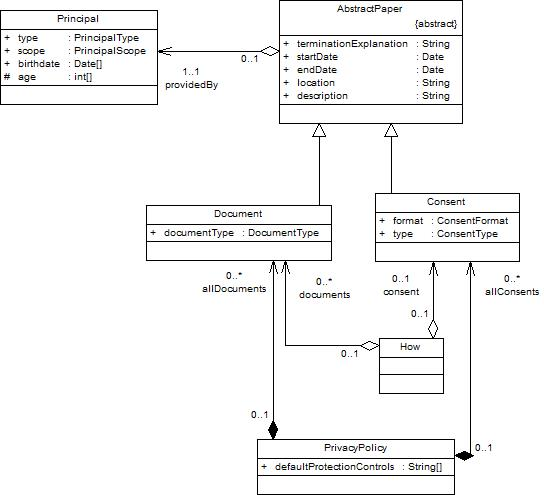
\includegraphics[width=10cm,scale=0.5]{images/document.jpg}
    \caption{Detailed view of the document entities}
    \label{fig:Document}
\end{figure}
\subsubsection{Data owner rights}
The Complaint describes each type of user complaint prescribed by the GDPR. It provides information about when does complaint happened and the reason for the complaint. Article 7 defines the withdrawal of consent. The data owner can withdraw the previously given consent for data processing at any time. The set of GDPR Articles 12 - 23 deals with data rights. Articles 16 and 17 provide the owner's rights to rectification and erasure of data. Article 18 allows the data owner the right to restrict the processing. Based on these data owner rights, we modelled the following entities. \newline We modelled AbstractComplaintAction to more easily abstract the types of complaints. The Withdraw inherits the AbstractComplaintAction. We then defined an AbstractComplaint containing information on the complaint status. Articles 16, 17 and 18 determine the importance of the complaint status. They require that the processor executes the complaint as soon as possible unless Denial exists. The Denial contains information about the time, reason, and reference to the PrivacyPolices that are the cause of the rejection. The ComplaintBasedOnAction defines the right to restrict the processing, and the ComplaintBasedOnData specifies the rights to rectification and erasure of data.
\begin{figure}[H]
    \centering
    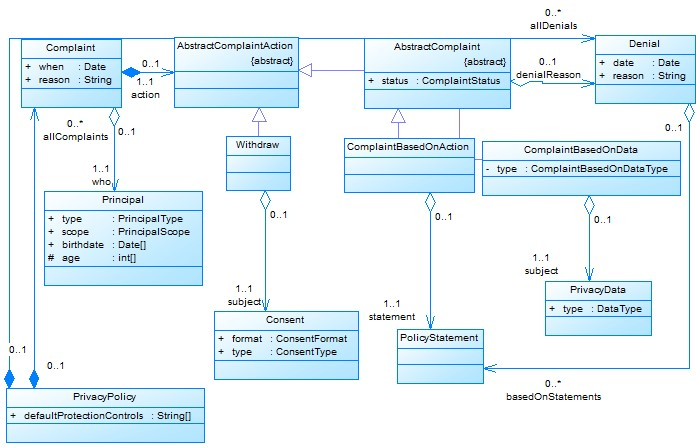
\includegraphics[width=10cm,scale=0.5]{images/dataRights.jpg}
    \caption{Detailed view of the data rights set of concepts}
    \label{fig:DataRights}
\end{figure}
\subsubsection{Notifications}
The NotificationInfo is an abstract class. Generalizes the types of actions in the system based on which the system creates user notifications. The GDPR quotes the Notifications as an essential functionality of the information system. Articles 19 and 33 define situations in which the system should notify data owners or data processors. There are two groups of notifications. The first one is data processing related, and the second one is complaint related. Consequently, PrivacyStatement and Complaint inherit the NotificationInfo. The Notification contains information about concrete Notification, such as date-time, NotificationType, receivers, notifiers and concrete action in the model that expresses the causedBy object. The NotifionType enumeration presents types of described notifications in Articles 19 and 33.
\begin{figure}[H]
    \centering
    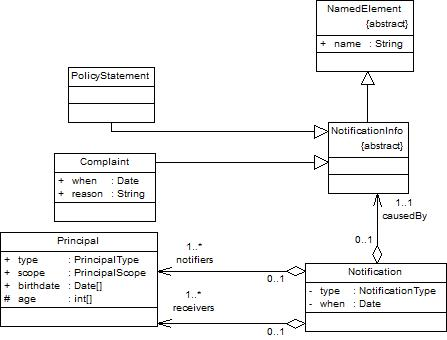
\includegraphics[width=10cm,scale=0.5]{images/notification.jpg}
    \caption{Detailed view of the notification set of concepts}
    \label{fig:Notifications}
\end{figure}
\subsubsection{Enumerations}
There is a detailed overview of all used enumerations.
\begin{figure}[H]
    \centering
    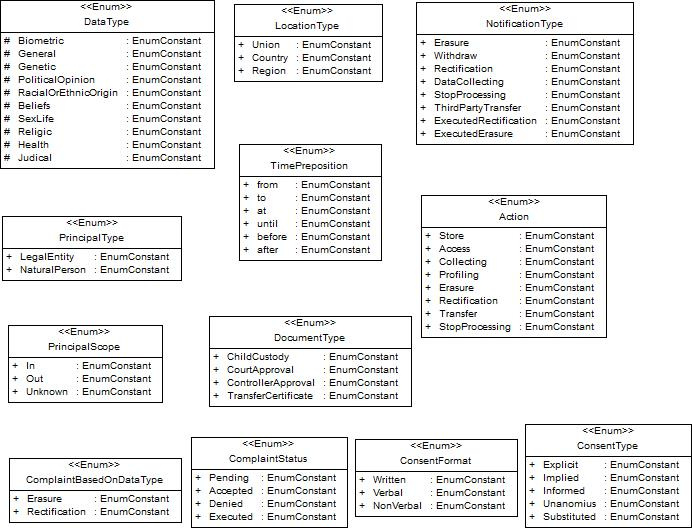
\includegraphics[width=12.5cm]{images/enums1.jpg}
    \caption{Detailed view of the used enums - part1}
    \label{fig:Enums1}
\end{figure}
\begin{figure}[H]
    \centering
    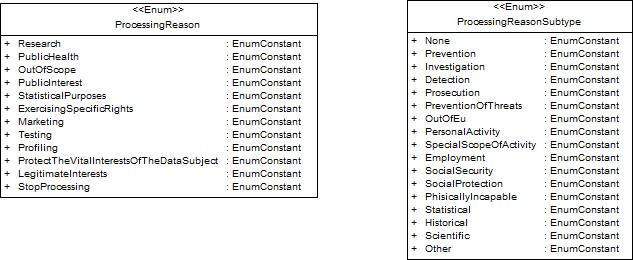
\includegraphics[width=12.5cm]{images/enums2.jpg}
    \caption{Detailed view of the used enums - part2}
    \label{fig:Enums2}
\end{figure}
\section{Case study}
We evaluated this meta-model against the example of the privacy policy of a real-world bank. We decided to describe these common business processes to show how flexible and clear the meta-model is to use in real life. Since we did not implement DSL, which we will discuss later, we used the existing xmi for verification, which is available in the development environment. To cover all the first 50 members of the GDPR, we made several use-cases. To simplify the example, the bank employs two workers: Ned Flanders and Patti Bouvier. \newline The first group of use cases deals with the opening of an account. This action is considered a rudimentary operation in the system since it collects information about the client. During data collection, the client defines the purpose for which the use of his data is allowed. In this case, the user, Edna Karabapel, wants to use data only for out of scope purposes and sub reason personal activity. For collecting data, it is necessary to submit consent. After that, Edna checked the status of the bank account. The bank officer accessed her data, so we tested Article 9. This Article checks whether the user has previously defined the purpose of data processing. To start the transfer, it is necessary to specify the transfer certificate, and it is also required that this document is valid. After the data transfer, the data processor should create a notification on the successful transfer of personal data. \newline The second group of use cases deals with the collection and processing of juvenile data. At first, we have tested Article 8. In case of collecting data on the child, the data processor should submit the document on custody of the child. As in the previous example, by collecting data, the owner defined all the purposes for data usage. Then, we tested the use of the child data. The third example has tested Article 16. It claims the rights of owners to submit a request to rectification their data. This article defines that it is necessary to carry out this complaint as soon as possible. After this, it is obligatory to inform the owner about the result, Article 19. The last example tested Article 17, which claims that the user has the privilege to file complaints about the use of data and requests their erasure. Also, it is necessary to process this request as soon as possible and inform the user about the result. 
\begin{figure}[H]
\centering
\begin{minipage}{.5\textwidth}
  \centering
  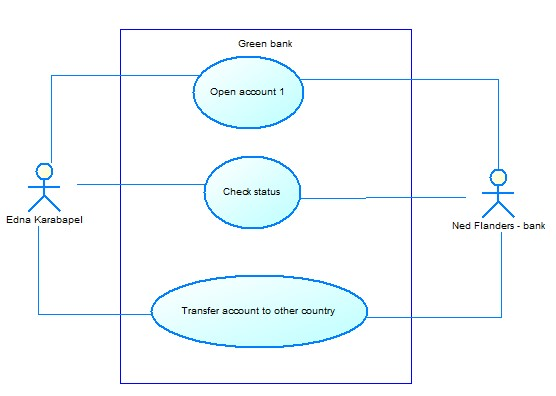
\includegraphics[width=6cm,scale=0.5]{images/use case1.jpg}
  \caption{Use case 1}
  \label{fig:usecase1}
\end{minipage}%
\begin{minipage}{.5\textwidth}
  \centering
  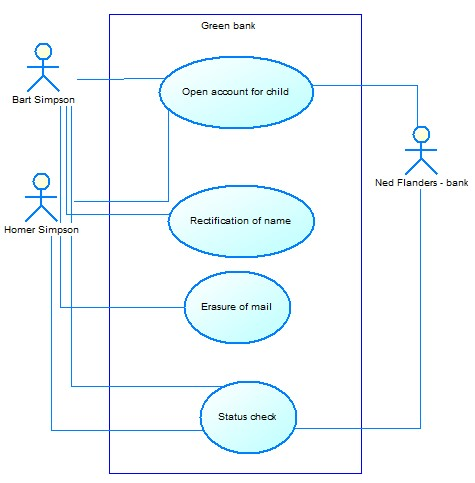
\includegraphics[width=6cm,scale=0.5]{images/use case2.jpg}
  \caption{Use case 2}
  \label{fig:usecase2}
\end{minipage}
\end{figure}
Through the third use case is tested Article 21, right to objection. In the first example, Homer permits the bank to use his data for marketing purposes. Then, they sent him an email to inform him about the new credit cards. Later, Homer complained about the email and want the bank to stop using his data for marketing purposes. \newline Through the fourth use case, we dealt with situations in which data owners are involved in some malicious actions. Therefore, it deals with data processing that requires the participation of legal entities, such as courts. In this example, Mr Burns was involved in illegal activities. Police came to the bank to check his account. Validation requires the police to submit a court authorization for access to user data, as Article 9 defines that the processing of such data requires a court authorization. This article also explicitly states, use for purposes of public interest is allowed. It is, therefore, necessary for the police to define the purpose of access to ownership data. Through these extensive four use cases, we tested the first 50 members of the GDPR.
\begin{figure}[H]
\centering
\begin{minipage}{.5\textwidth}
  \centering
  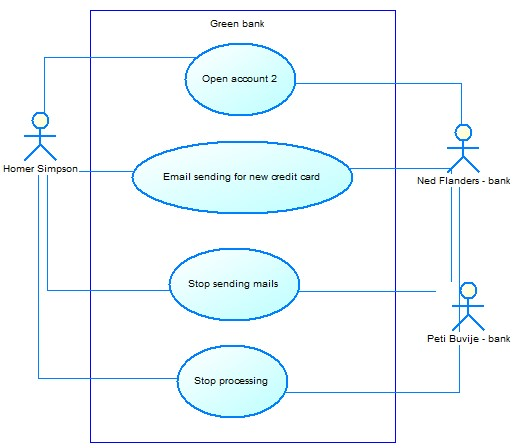
\includegraphics[width=6cm,scale=0.5]{images/use case3.jpg}
  \caption{Use case 3}
  \label{fig:usecase3}
\end{minipage}%
\begin{minipage}{.5\textwidth}
  \centering
  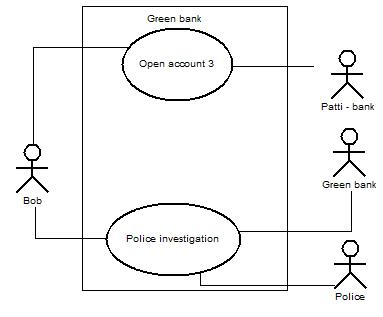
\includegraphics[width=6cm,scale=0.5]{images/use case4.jpg}
  \caption{Use case 4}
  \label{fig:usecase4}
\end{minipage}
\end{figure}
\section{Conclusion}
In this paper, we propose and discuss a meta-model for verifying GDPR violations. We used EMF Framework, UML and OCL to develop this meta-model. The prime motivation for this research is to provide unambiguous and plain language close to natural language. The idea is to make this language understandable to software engineers and legal experts to make it easier to interpret the GDPR and bridge the communication gap. \newline As our focus was on flexibility and simplicity, we wanted to show through the Case study section that it is possible to describe complex actions in banking systems with this meta-model. This case study shows the potential for this meta-model. Companies can use it to express privacy requirements in existing business systems. We have covered the first 50 articles to cover all potential actions in the business system that affect a specific company. The other 50 articles handle legal institutions. We have not processed them since the daily work does not require them. \newline This meta-model is just the basis for developing automated validation. We have not developed a domain-specific language because we do not want to use graphic or text notations. Instead of developing the language, we want to define annotations that developers will later include into existing applications. Then, with the help of aspect-oriented programming, we will read the annotations in real-time and create a model over which we will perform validation. After changing the model, we will create a report and notify the user if it violates a GDPR article. The unified solution would solve many of the problems we talked about at the beginning of the paper. Primarily, companies will reduce costs, as there would be no need to develop a specific solution for each system. In addition, it will be possible to integrate annotations with existing software solutions.
\printbibliography
\end{document}